% secciones/métodos.tex
\section{Materiales y métodos}
\label{sec:metodos}

\subsection{Sistema experimental y protocolo de medición}
\label{sec:sistema}

Los experimentos se realizaron en recipientes plásticos rígidos de geometría
troncopiramidal rectangular: boca superior de $37 \times 26$~cm, base de
$32 \times 21$~cm y altura de $17$~cm, para un volumen geométrico de
$\approx 13{,}8$~L. Los sensores de gases (CO$_2$, MH-410D; CH$_4$, MH-440D)
se montaron empotrados en una de las caras laterales mayores, con el elemento
sensible hacia el interior y por encima del nivel del sustrato. Durante cada
cierre el recipiente se mantuvo sellado con su tapa reforzada con silicona, y
el volumen de aire efectivo $V_{\mathrm{aire}}$ ---el volumen geométrico menos
el ocupado por el recipiente interno y su contenido--- entró como parámetro
medido en el cálculo de tasas.

El sustrato y las larvas se alojaron en un recipiente plástico de
$15 \times 12 \times 5$~cm con tapa aireada por malla, colocado dentro de la
cámara; se supuso equilibrio rápido de gases entre el recipiente interno y el
aire de la cámara a través de la malla. El mismo tipo de montaje se usó en
tratamientos y controles, de modo que $V_{\mathrm{aire}}$ fue comparable entre
ellos.

Se evaluaron dos dietas, D1 y D4, cuya composición se detalla en la
Cuadro~\ref{tab:dietas}. En cada día de medición los cierres se realizaron de
forma secuencial por dieta: primero un recipiente hasta la saturación del
sensor de CO$_2$ (6000~ppm) y luego el otro, con el mismo procedimiento. Cada
condición se midió con tres cierres consecutivos sobre el mismo lote (réplicas técnicas de medición); el valor reportado por punto es su media y el rango su dispersión. Las réplicas biológicas (lotes independientes) quedan como extensión futura. Como controles se incluyeron
recipientes con alimento solo (respiración del sustrato) y con larvas solas
(mantenimiento sin alimento), medidos con el mismo protocolo; la tasa neta de
cada tratamiento se obtuvo restando el control correspondiente del mismo día.

Cada lote se cargó una sola vez al inicio del ciclo, sin reposición ni
retiro: 250~g de sustrato por recipiente, preparado mezclando el
alimento seco con agua hasta una humedad del 70~\% en base húmeda
(75~g de materia seca y 175~g de agua), y 700 larvas por tratamiento.
Los controles de alimento solo llevaron los mismos 250~g de sustrato
sin larvas. La temperatura dentro de la cámara se registró de forma
continua y se mantuvo aproximadamente constante entre cierres.

La tasa de cada cierre se estimó por ajuste lineal del tramo previo a la
saturación; cuando el ajuste fue de baja calidad o la curva alcanzó el techo
del sensor (cierres marcados como saturados), la tasa estimada es conservadora
y se trató como cota inferior en la validación (sec. \ref{sec:resultados}).

\begin{table}[htbp]
  \centering
  \caption{Descripción de las dietas evaluadas.}
  \label{tab:dietas}
  \begin{tabular}{lp{8cm}}
    \hline
    Dieta & Descripción \\
    \hline
    D1 & Alimento comercial estándar para pollo de engorde (dieta de
         referencia del modelo de Eriksen) \\
    D4 & Residuos agroindustriales de frutas (naranja, plátano, entre
         otras), fermentados \\
    \hline
  \end{tabular}
\end{table}

\subsection{Modelo dinámico del proceso}
\label{sec:modelo}

El proceso se describe con un modelo dinámico de parámetros concentrados (0D) que amplia el modelo de asimilación, crecimiento y producción de CO$_2$ de \textcite{eriksenDynamicModellingFeed2022,eriksenMetabolicPerformanceFeed2024} (en adelante, el \emph{modelo de referencia}) ---desarrollado para larvas de \textit{H. illucens} sobre dieta estándar--- con tres componentes adicionales: (i) un interruptor de prepupa que representa la cesación de la alimentación al final del ciclo larvario; (ii) un módulo microbiano de primer orden para la degradación del sustrato no consumido \parencite{roels1980}; y (iii) un balance de masa de gas en la cabeza de aire de la cámara estática de medición. Los fundamentos de la teoría DEB del núcleo larvario se encuentran en \parencite{kooijmanDynamicEnergyBudget2009,jagerDEBkissQuestSimplest2013}. El modelo supone temperatura constante (medida) y humedad del lecho como variable de estado, oxígeno no limitante dentro de los cierres y número de larvas $N$ constante (mortalidad despreciable en el periodo experimental).

El vector de estado es $\mathbf{x} = (A, B, L, D_M, W, X, c_{CO_2}, c_{CH_4})$, donde $A$, $B$ y $L$ son los compartimentos larvarios (asimilado, estructura y lípidos, mg/larva), $D_M$, $W$ y $X$ la materia seca, el agua y la biomasa microbiana del lecho (g), y $c_i$ las concentraciones de gas en la cabeza de aire (mol/m$^3$). Las condiciones iniciales $A_0 = 0.005$ y $L_0 = 0.003$~mg corresponden a una larva neonata \parencite{eriksenDynamicModellingFeed2022}; $B_0$ se calibró en este trabajo con las tasas netas (Cuadro~\ref{tab:parametros}).

\subsubsection{Núcleo larvario (DEB de Eriksen)}

El núcleo sigue el modelo de compartimentos de \textcite{eriksenDynamicModellingFeed2022}: el alimento asimilado entra al compartimento $A$ y de allí se reparte entre crecimiento estructural $B$, reservas lipídicas $L$ y costos metabólicos pagados como CO$_2$ (Figura \ref{fig:nucleo}); los fundamentos DEB de esta partición están en \parencite{kooijmanDynamicEnergyBudget2009}. A continuación se indica la procedencia de cada expresión.

\begin{figure}[htbp]
\centering
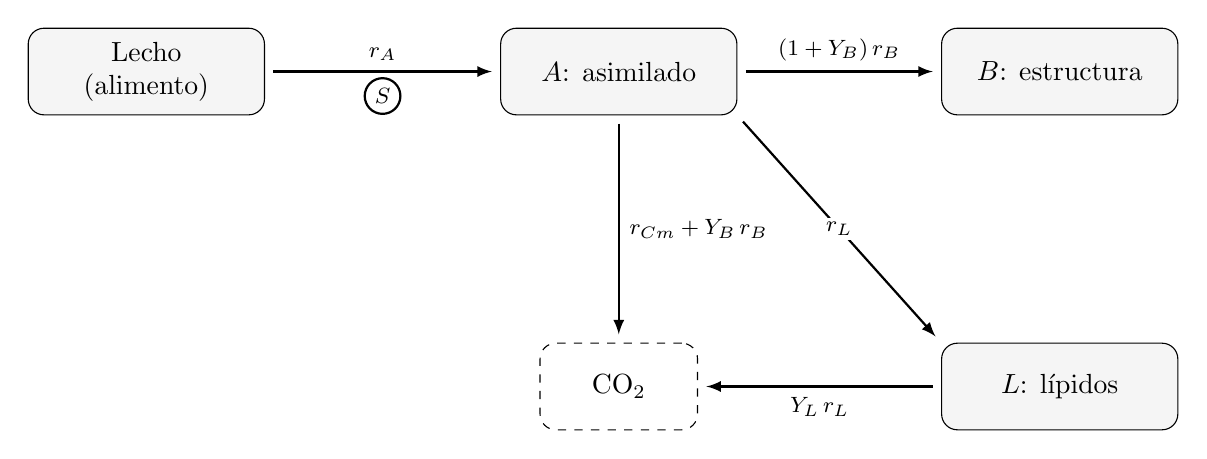
\begin{tikzpicture}[
  comp/.style={draw, rounded corners=2mm, minimum width=3.0cm, minimum height=1.1cm, align=center, fill=gray!8},
  gas/.style={draw, dashed, rounded corners=2mm, minimum width=2.0cm, minimum height=1.1cm, align=center},
  gate/.style={circle, draw, thick, fill=white, inner sep=1.8pt, font=\footnotesize},
  flujo/.style={->, >=latex, thick, shorten >=3pt, shorten <=3pt},
  etiqueta/.style={fill=white, inner sep=1.5pt, font=\footnotesize}]
\node[comp] (alim) at (0,0) {Lecho\\ (alimento)};
\node[comp] (A) at (6.0,0) {$A$: asimilado};
\node[comp] (B) at (11.6,0) {$B$: estructura};
\node[comp] (L) at (11.6,-4.0) {$L$: lípidos};
\node[gas] (CO2) at (6.0,-4.0) {CO$_2$};
\draw[flujo] (alim) -- node[etiqueta, above=2pt]{$r_A$}
                      node[gate, below=2pt]{$S$} (A);
\draw[flujo] (A) -- node[etiqueta, above=2pt]{$(1 + Y_B)\,r_B$} (B);
\draw[flujo] (A) -- node[etiqueta, right=2pt]{$r_{Cm} + Y_B\,r_B$} (CO2);
\draw[flujo] (A.south east) -- node[etiqueta]{$r_L$} (L.north west);
\draw[flujo] (L) -- node[etiqueta, below=2pt]{$Y_L\,r_L$} (CO2);
\end{tikzpicture}
\caption{Compartimentos y flujos de carbono del núcleo larvario (adaptado de \parencite{eriksenDynamicModellingFeed2022}). El interruptor de prepupa $S(t)$ (ecuación \ref{eq:prepupa}) cierra la entrada de alimento al final del ciclo; los costos $r_{Cm}$, $Y_B r_B$ y $Y_L r_L$ salen del sistema como CO$_2$.}
\label{fig:nucleo}
\end{figure}

\paragraph{Interruptor de prepupa (extensión respecto al modelo de referencia).}
Al final del último instar, las larvas de \textit{H. illucens} cesan la
alimentación y entran en prepupa, un estadio de transición a la metamorfosis
en el que el insecto no se alimenta y sostiene su metabolismo con las reservas
acumuladas durante la fase larvaria, principalmente los lípidos del cuerpo
graso \parencite{arreseInsectFatBody2010,nayakHermetiaIllucensDiptera2023}.
Fisiológicamente, la transición es un umbral del ciclo de vida: en los modelos
DEB de insectos holometábolos, los cambios de estadio separan regímenes
energéticos distintos, con asimilación en la fase larvaria y metabolismo de
mantenimiento sobre reservas en las fases no alimentarias
\parencite{kooijmanDynamicEnergyBudget2009,llandresDynamicEnergyBudget2015}.
El modelo de \textcite{eriksenDynamicModellingFeed2022} no incluye este
cierre, por lo que predice asimilación y producción de CO$_2$ sostenidas al
final del ciclo, en contradicción con el colapso de las emisiones observado
entre los días 13 y 17 (sec. \ref{sec:resultados}).

Para representarlo, se introduce la fracción de la cohorte que sigue
alimentándose como una función del tiempo. La forma no es arbitraria: en una
cohorte de $N \approx 700$ larvas la entrada a prepupa no es sincrónica, y si
los tiempos individuales de transición se distribuyen alrededor de un día
central $t_p$ con dispersión $w_p$, la fracción de larvas aún en alimentación
es la función de supervivencia de esa distribución. Para una distribución
logística de los tiempos de transición, dicha fracción es
\begin{equation}
S(t) = \frac{1}{1 + \exp(-(t - t_p)/w_p)},
\label{eq:prepupa}
\end{equation}
con $S \to 1$ al inicio del ciclo (toda la cohorte alimentándose) y $S \to 0$
al final (toda la cohorte en prepupa). El parámetro $t_p$ es el día central de
la transición y $w_p$ su anchura, interpretable como la sincronía de la
cohorte: el límite $w_p \to 0$ corresponde a una transición perfectamente
sincrónica (un interruptor ideal), que sería discontinuo, no estimable con
mediciones diarias y numéricamente rígido; la versión suave es diferenciable y
monótona decreciente, lo que mantiene el campo vectorial continuo para la
integración (sec. 2.3). En el modelo, el factor $(1 - S(t))$ cierra la
asimilación (ec. \ref{eq:asimilacion}) y el suelo de mantenimiento
$m_{\mathrm{suelo}}$ representa el metabolismo residual sobre reservas durante
la prepupa, anclado a la medición de larvas en ayuno (sec. 3). Los parámetros
$t_p$ y $w_p$ se ajustan al descenso de las tasas medidas entre los días 13 y
17.

\paragraph{Asimilación (ecs. 4 y 5 de Eriksen, 2022).}
La tasa específica de asimilación decrece con el tamano y el flujo asimilado es proporcional a $B$ \parencite{eriksenDynamicModellingFeed2022}:
\begin{equation}
a(B, t, D_M) = f\,a_{\max}\,\frac{1}{1 + (B/B_{\max})^{\alpha}}\,(1 - S(t))\,\frac{D_M}{D_M + K_s},
\qquad r_A = a\,B,
\label{eq:asimilacion}
\end{equation}
donde $B_{\max}$ es la biomasa de referencia y $\alpha$ controla la caida con el tamano. El factor $(1 - S(t))$ es el interruptor de prepupa de la ec. \ref{eq:prepupa}: cierra la asimilación al final del ciclo. También son extensiones respecto al modelo de referencia el factor de calidad de dieta $f$ ($f = 1$ en D1, calibrado en D4, sec. \ref{sec:resultados}) y la limitación por disponibilidad de alimento $D_M/(D_M + K_s)$, con $K_s = 2$~g fijo, que apaga la asimilación suavemente cuando el sustrato se agota en el régimen de carga única.

\paragraph{Crecimiento (ec. 10 de Eriksen, 2022).}
El crecimiento estructural sigue la forma logistica con descuento de mantenimiento de \textcite{eriksenDynamicModellingFeed2022}:
\begin{equation}
G(B) = \max\!\left(1 - (B/B_{\max})^{\beta}, 0\right),
\qquad
\mu_B = \max\!\left(\frac{(a - m)\,G}{1 + Y_B\,G}, 0\right),
\qquad r_B = \mu_B\,B,
\label{eq:crecimiento}
\end{equation}
donde $m$ es la tasa de mantenimiento específico, en la tradición de Pirt y los principios macroscopicos de \textcite{roels1980}, y $Y_B$ el costo de crecimiento.

\paragraph{Mantenimiento (Eriksen, 2022, con suelo de prepupa).}
El costo de mantenimiento es proporcional a la estructura, y durante la prepupa cae a un suelo añadido en este trabajo, anclado a la medición de larvas en ayuno del día 17 (sec. \ref{sec:resultados}):
\begin{equation}
r_{Cm} = m\,B\,\big[(1 - S(t)) + m_{\mathrm{suelo}}\,S(t)\big].
\label{eq:mantenimiento}
\end{equation}

\paragraph{Balance de lípidos y CO$_2$ (ec. 12 de Eriksen, 2022).}
Suponiendo el compartimento $A$ en cuasi-equilibrio ($dA/dt \approx 0$), lo asimilado se reparte instantaneamente entre crecimiento, mantenimiento y reservas, lo que da el flujo neto a lípidos y la producción larvaria de CO$_2$ como la suma de los tres costos respiratorios \parencite{eriksenDynamicModellingFeed2022,eriksenMetabolicPerformanceFeed2024}:
\begin{equation}
r_L = r_A - (1 + Y_B)\,r_B - r_{Cm},
\qquad
r_{CO_2}^{\mathrm{lar}} = r_{Cm} + Y_B\,r_B + Y_L\,\max(r_L, 0),
\label{eq:co2lar}
\end{equation}
con $Y_L$ el costo de depósito de lípidos; todas las tasas en mg/larva/d.

\subsubsection{Módulo microbiano del lecho}
En la bioconversión, las larvas no consumen la totalidad del sustrato: la
fracción no asimilada permanece en el lecho, donde es descompuesta por la
microbiota ambiental en paralelo al consumo larvario (Figura
\ref{fig:lecho}). Esta fuente no es despreciable: las emisiones medidas en
reactores con \textit{H. illucens} mezclan la respiración larvaria y la
microbiana \parencite{ermolaevGreenhouseGasEmissions2019,parodiBioconversionEfficienciesGreenhouse2020a},
y en los controles de alimento solo de este experimento las tasas de CO$_2$
aumentaron de forma sostenida a lo largo del ciclo (sec.
\ref{sec:resultados}). Una cinética de primer orden sobre la materia seca no
puede reproducir ese aumento, pues el sustrato solo decrece; la explicación
microbiológica es el crecimiento de la propia biomasa degradadora. Por ello,
la segunda extensión respecto al modelo de referencia representa la biomasa
microbiana $X$ como un estado que crece sobre el sustrato degradado, en la
tradición de los balances macroscópicos de la ingeniería bioquímica
\parencite{roels1980,shulerbioprocess2017}. A continuación se indica la
procedencia de cada expresión.

\begin{figure}[htbp]
\centering
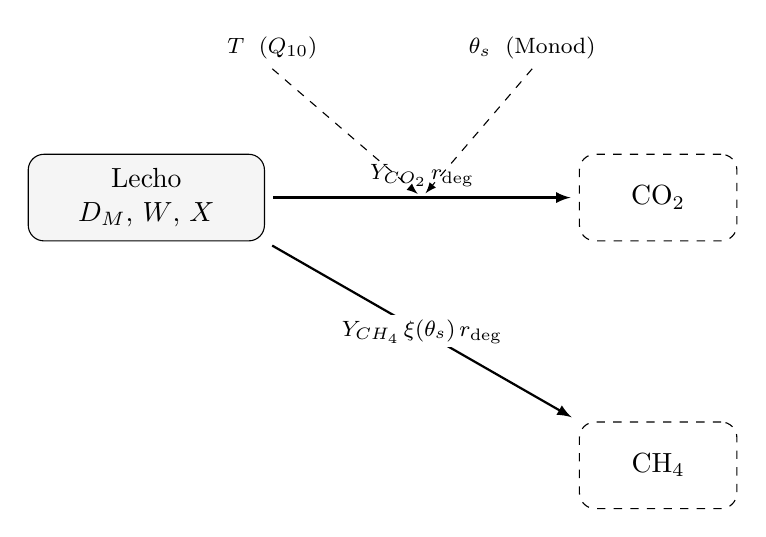
\begin{tikzpicture}[
  comp/.style={draw, rounded corners=2mm, minimum width=3.0cm, minimum height=1.1cm, align=center, fill=gray!8},
  gas/.style={draw, dashed, rounded corners=2mm, minimum width=2.0cm, minimum height=1.1cm, align=center},
  drv/.style={font=\footnotesize, align=center},
  flujo/.style={->, >=latex, thick, shorten >=3pt, shorten <=3pt},
  mod/.style={->, >=latex, dashed, shorten >=2pt},
  etiqueta/.style={fill=white, inner sep=1.5pt, font=\footnotesize}]
\node[comp] (lecho) at (0,0) {Lecho\\ $D_M$, $W$, $X$};
\node[gas] (co2) at (6.5,0) {CO$_2$};
\node[gas] (ch4) at (6.5,-3.4) {CH$_4$};
\node[drv] (T) at (1.6,1.9) {$T$\; ($Q_{10}$)};
\node[drv] (H) at (4.9,1.9) {$\theta_s$\; (Monod)};
\draw[flujo] (lecho) -- node[etiqueta, above=2pt]{$Y_{CO_2}\,r_{\mathrm{deg}}$}
                       node[coordinate, pos=0.5] (k) {} (co2);
\draw[flujo] (lecho.south east) -- node[etiqueta]{$Y_{CH_4}\,\xi(\theta_s)\,r_{\mathrm{deg}}$} (ch4.north west);
\draw[mod] (T.south) -- (k);
\draw[mod] (H.south) -- (k);
\end{tikzpicture}
\caption{Módulo microbiano del lecho (extensión respecto al modelo de referencia). La constante efectiva $k$ (ec. \ref{eq:kmic}) integra la corrección térmica $Q_{10}$ y la respuesta de humedad tipo Monod; la degradación $r_{\mathrm{deg}}$ (ec. \ref{eq:rmic}) crece con la biomasa microbiana $X$ y se apaga al agotarse el sustrato; el CH$_4$ se activa con la fracción saturada $\theta_s$ via $\xi$, como indicador cualitativo.}
\label{fig:lecho}
\end{figure}

\paragraph{Humedad del lecho y constante efectiva (formas estándar, combinadas en este trabajo).}
La actividad microbiana depende de la temperatura y de la humedad del lecho,
ambas documentadas como factores de control del proceso con \textit{H.
illucens} \parencite{bekkerImpactSubstrateMoisture2021a,mertenatBlackSoldierFly2019}.
El estado de humedad se resume en la fracción gravimétrica $\theta_s =
W/(D_M + W)$, la cantidad medible en el experimento (carga inicial de 75~g
de materia seca y 175~g de agua, es decir $\theta_s = 0.7$). La constante
efectiva de degradación combina tres elementos clásicos de la cinética de
descomposición de residuos \parencite{roels1980,shulerbioprocess2017}: una
corrección térmica tipo van 't Hoff, en la que la tasa se multiplica por
$Q_{10}$ cada 10~°C respecto a una temperatura de referencia $T_{\mathrm{ref}}$;
una respuesta de saturación a la humedad tipo Monod con semisaturación
$K_{\theta}$; y un tope $k_{\max}$ no limitante, incluido solo por seguridad
numérica:
\begin{equation}
k = \min\!\left(k_{\mathrm{ref}}\,Q_{10}^{(T - T_{\mathrm{ref}})/10}\,
\frac{\theta_s}{\theta_s + K_{\theta}},\; k_{\max}\right),
\label{eq:kmic}
\end{equation}
Los valores $Q_{10} = 2$ y $T_{\mathrm{ref}} = 25$~°C son nominales estándar
\parencite{roels1980,shulerbioprocess2017}; $K_{\theta} = 0.15$ y $k_{\max} =
1.0$~d$^{-1}$ son valores fijos no calibrados. Como $\theta_s \approx 0.7 \gg
K_{\theta}$ durante todo el ensayo, la humedad no fue limitante y el factor
$\theta_s/(\theta_s + K_{\theta})$ operó cerca de la saturación; su papel es
estructural, para condiciones más secas. El único parámetro cinético calibrado
es $k_{\mathrm{ref}}$ (sec. \ref{sec:resultados}).

\paragraph{Tasas de CO$_2$ y CH$_4$ microbianos.}
Desde el punto de vista químico, la degradación microbiana del lecho es la
oxidación de la materia orgánica residual: los microorganismos usan el
sustrato como fuente de carbono y energía, liberan CO$_2$ como producto
final de la respiración e incorporan una fracción del carbono a biomasa
nueva. La tasa de degradación $r_{\mathrm{deg}}$, en gramos de sustrato
degradado por día, se toma proporcional a la biomasa microbiana $X$ que
cataliza el proceso y limitada por el sustrato disponible mediante una forma
de Monod con semisaturación $K_{sm}$: con sustrato abundante la tasa satura
en $k\,X$ (la capacidad máxima de la biomasa presente), y cuando el sustrato
se agota, la tasa tiende a cero de forma continua. Este término fue añadido en este trabajo, con $K_{sm} = 5$~g fijo y no calibrado: es pequeño frente a la carga inicial ($D_M(0) = 75$~g), de modo que el factor opera cerca de la saturación durante la ventana de medición y su valor exacto no afecta los resultados; su papel es dar un apagado continuo de la degradación al agotarse el sustrato. El CO$_2$ microbiano se obtiene con un rendimiento
$Y_{CO_2}$ sobre el sustrato degradado, en la tradición de los balances
macroscópicos \parencite{roels1980,shulerbioprocess2017}; $Y_{CO_2}$ se
calibra contra los controles (sec. \ref{sec:resultados}).

El CH$_4$ tiene un origen distinto: la metanogénesis es un proceso anaerobio
estricto que, en un lecho húmedo y bien aireado en promedio, solo puede
ocurrir en microambientes anóxicos, asociados a las zonas saturadas de agua;
de ahí que las emisiones de CH$_4$ reportadas en bioconversión con
\textit{H. illucens} dependan del sustrato y de las condiciones de humedad
\parencite{ermolaevGreenhouseGasEmissions2019,parodiBioconversionEfficienciesGreenhouse2020a,boakye-yiadomGreenhouseGasEmissions2022}.
El término, introducido en este trabajo, modula la tasa con un factor
logístico $\xi(\theta_s)$ de la fracción saturada: $\xi$ es prácticamente
nulo a humedades moderadas y crece al acercarse el lecho a la saturación.
Este término se usa solo como indicador cualitativo, pues el sensor
disponible no está calibrado para tasa neta
\parencite{mitchellCalibrationLowCostMethane2024,kiplimoAddressingLowCostMethane2024}.
Los parámetros de $\xi$ ($\theta_{cs}$, $s_\theta$, $\xi_{\max}$) y
$Y_{CH_4}$ son nominales, no calibrados, y el término no entra en la
validación cuantitativa.

\begin{equation}
\begin{aligned}
r_{\mathrm{deg}} &= k\,X\,\frac{D_M}{D_M + K_{sm}},
&
r_{C}^{\mathrm{mic}} &= Y_{CO_2}\,r_{\mathrm{deg}},
\\
r_{CH_4} &= Y_{CH_4}\,\xi(\theta_s)\,r_{\mathrm{deg}},
&
\xi(\theta_s) &= \frac{\xi_{\max}}{1 + \exp(-(\theta_s - \theta_{cs})/s_{\theta})},
\end{aligned}
\label{eq:rmic}
\end{equation}
en g/d.

\paragraph{Biomasa microbiana (estado añadido en este trabajo).}
Al degradar el sustrato, los microorganismos incorporan una fracción del
carbono a biomasa nueva: el crecimiento microbiano es proporcional a la tasa
de degradación, con un rendimiento $Y_X$ (gramos de biomasa formada por gramo
de sustrato degradado), concepto estándar de la cinética de cultivos
\parencite{roels1980,shulerbioprocess2017}:
\begin{equation}
\frac{dX}{dt} = Y_X\,r_{\mathrm{deg}},
\qquad X(0) = X_0.
\label{eq:xmic}
\end{equation}
Sin mediciones directas de biomasa, las curvas de control solo informan dos
combinaciones de parámetros: el nivel inicial de la tasa, $Y_{CO_2}\,k\,X_0$,
y la tasa de crecimiento aparente, $\mu = Y_X\,k$. Por ello no es posible
estimar $X_0$, $Y_X$ y $k$ por separado: se fijan $X_0 = 1$~g (valor nominal,
con lo que la trayectoria de $X$ queda en unidades nominales y lo que
informan los datos es el producto $k\,X$) y $Y_X = 0.4$ (rendimiento aerobio
típico sobre carbohidratos \parencite{roels1980}), y se calibran
$k_{\mathrm{ref}}$ e $Y_{CO_2}$ contra los controles (sec.
\ref{sec:resultados}).

\paragraph{Balance de masa del lecho.}
El lecho pierde materia seca por dos vías ya formuladas: el consumo
larvario ($N\,r_A/1000$, en g/d, ec. \ref{eq:asimilacion}) y la
degradación microbiana ($r_{\mathrm{deg}}$, definida en el párrafo
anterior). A la vez gana agua: la oxidación de carbohidratos libera un
mol de H$_2$O por cada mol de CO$_2$ producido
\parencite{atkinsPhysicalChemistry2014}, de modo que la respiración
larvaria y microbiana aporta agua metabólica al lecho en proporción
fija $\gamma_w = 18/44 \approx 0.41$~g de H$_2$O por g de CO$_2$.
La evaporación se desprecia a la escala de los cierres (minutos) y la
pérdida por ventilación entre cierres no se modela; ambas se declaran
como limitaciones del balance de agua.
\begin{equation}
\frac{dD_M}{dt} = -\frac{N\,r_A}{1000} - r_{\mathrm{deg}},
\qquad
\frac{dW}{dt} = \gamma_w\left(\frac{N\,r_{CO_2}^{\mathrm{lar}}}{1000} + r_C^{\mathrm{mic}}\right),
\qquad
\frac{dX}{dt} = Y_X\,r_{\mathrm{deg}},
\label{eq:lecho}
\end{equation}
El tope $D_M \geq 0$ impide sustrato negativo, y la ecuación de $X$
se repite de la ec. \ref{eq:xmic} para dejar el sistema del lecho
completo en una sola expresión. El experimento fue de carga única: se
pusieron 250~g de sustrato al inicio (75~g de materia seca y 175~g de
agua, relación 30/70) y no hubo reposición ni retiro durante el ciclo,
de modo que $D_M(0) = 75$~g y $W(0) = 175$~g son las condiciones
iniciales del lecho.

\subsubsection{Balance de gas en cámara estática}

El tercer componente conecta las fuentes con la medición: durante un cierre, el CO$_2$ y el CH$_4$ se acumulan en el volumen de aire de la cámara y el sensor registra la pendiente de concentración (Figura \ref{fig:camara}).

\begin{figure}[htbp]
\centering
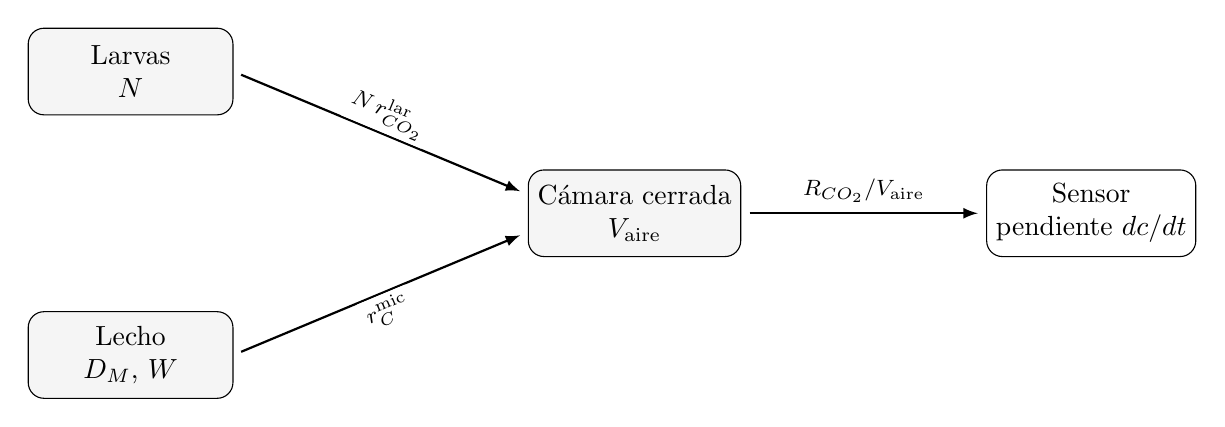
\begin{tikzpicture}[
  comp/.style={draw, rounded corners=2mm, minimum width=2.6cm, minimum height=1.1cm, align=center, fill=gray!8},
  inst/.style={draw, rounded corners=2mm, minimum width=2.6cm, minimum height=1.1cm, align=center},
  flujo/.style={->, >=latex, thick, shorten >=3pt, shorten <=3pt},
  etiqueta/.style={fill=white, inner sep=1.5pt, font=\footnotesize}]
\node[comp] (larvas) at (0,1.8) {Larvas\\ $N$};
\node[comp] (lecho) at (0,-1.8) {Lecho\\ $D_M$, $W$};
\node[comp] (cámara) at (6.4,0) {Cámara cerrada\\ $V_{\mathrm{aire}}$};
\node[inst] (sensor) at (12.2,0) {Sensor\\ pendiente $dc/dt$};
\draw[flujo] (larvas.east) -- node[etiqueta, sloped, above]{$N\,r_{CO_2}^{\mathrm{lar}}$} (cámara.170);
\draw[flujo] (lecho.east) -- node[etiqueta, sloped, below]{$r_C^{\mathrm{mic}}$} (cámara.190);
\draw[flujo] (cámara) -- node[etiqueta, above=2pt]{$R_{CO_2}/V_{\mathrm{aire}}$} (sensor);
\end{tikzpicture}
\caption{Balance de gas en la cámara estática, sobre el método estándar \parencite{hutchinsonMethodsSoilAnalysis1992}. Las fuentes larvaria y microbiana acumulan gas en el volumen de aire durante un cierre (ec. \ref{eq:camara}); el sensor registra la pendiente, llevada a ppm/min con la ley de gas ideal (ec. \ref{eq:ppm}).}
\label{fig:camara}
\end{figure}

\paragraph{Acumulación en el cierre (balance de este trabajo sobre el método estándar).}
El método de cámara estática estima la tasa a partir de la acumulación lineal del gas en un volumen conocido \parencite{hutchinsonMethodsSoilAnalysis1992}; con las fuentes del modelo, el balance molar sobre el aire de la cámara es
\begin{equation}
\frac{dc_{CO_2}}{dt} = \frac{R_{CO_2}}{V_{\mathrm{aire}}},
\qquad
R_{CO_2} = \frac{N\,r_{CO_2}^{\mathrm{lar}} + 1000\,r_C^{\mathrm{mic}}}{44000},
\label{eq:camara}
\end{equation}
con $R_{CO_2}$ en mol/d: el término larvario pasa de mg a g y ambos a mol con la masa molar del CO$_2$ (44 g/mol); un balance análogo aplica para $c_{CH_4}$ con $R_{CH_4} = 1000\,r_{CH_4}/16000$ (16 g/mol).

\paragraph{Escala del sensor (ppm/min).}
La comparación con el sensor se hace en la escala propia del método \parencite{hutchinsonMethodsSoilAnalysis1992}, convirtiendo la acumulación molar a ppm/min con la ley de gas ideal \parencite{atkinsPhysicalChemistry2014}:
\begin{equation}
r_{\mathrm{ppm}} = \frac{R_{CO_2}}{V_{\mathrm{aire}}}\,\frac{R_g\,T}{P}\,\frac{10^6}{1440}
\quad [\mathrm{ppm/min}],
\label{eq:ppm}
\end{equation}
con $R_g = 8.314$ J/(mol$\cdot$K) y $T$, $P$ la temperatura y presión de la cámara: el factor $R_g T/P$ es el volumen molar, $10^6$ lleva a ppm y 1440 de días a minutos.

\paragraph{Validación por descomposición de fuentes (estrategia de este trabajo).}
La validación explota la descomposición de fuentes: la componente larvaria $N\,r_{CO_2}^{\mathrm{lar}}$ se compara con la tasa neta medida (tratamiento menos control del mismo día, promedio de tres cierres consecutivos), y la componente microbiana $r_C^{\mathrm{mic}}$ con las curvas de control (alimento solo). Los parámetros del núcleo DEB se tomaron de \textcite{eriksenDynamicModellingFeed2022,eriksenMetabolicPerformanceFeed2024} (Cuadro \ref{tab:parametros}); los del módulo microbiano ($k_{\mathrm{ref}}$, $Y_{CO_2}$) se calibran en este trabajo contra las curvas de control (sec. \ref{sec:resultados}).

\begin{table}[htbp]
\centering
\caption{Parámetros del modelo. Núcleo DEB: literatura (ver texto). Interruptor de prepupa, $B_0$ y $f$: calibrados en este trabajo con las tasas netas (sec. \ref{sec:resultados}). Módulo microbiano: $k_{\mathrm{ref}}$ e $Y_{CO_2}$ calibrados con los controles (sec. \ref{sec:resultados}); demás parámetros fijos. Cámara: mediciones del experimento.}
\label{tab:parametros}
\begin{tabular}{llll}
\toprule
Parámetro & Símbolo & Valor & Unidad \\
\midrule
Tasa máxima de asimilación & $a_{\max}$ & 1.4 & d$^{-1}$ \\
Exponente de asimilación & $\alpha$ & 1.0 & -- \\
Exponente de crecimiento & $\beta$ & 2.0 & -- \\
Costo de crecimiento & $Y_B$ & 0.44 & -- \\
Costo de depósito de lípidos & $Y_L$ & 0.42 & -- \\
Mantenimiento & $m$ & 0.08 & d$^{-1}$ \\
Biomasa de referencia & $B_{\max}$ & 65 & mg \\
Día central de prepupa & $t_p$ & 16.4 (D1), 12.1 (D4) & d \\
Ancho del interruptor & $w_p$ & 0.36 & d \\
Suelo de mantenimiento & $m_{\mathrm{suelo}}$ & 0.13 & -- \\
Biomasa inicial por larva & $B_0$ & 0.0735 & mg \\
Factor de calidad de dieta & $f$ & 1 (D1), 0.698 (D4) & -- \\
Número de larvas & $N$ & 700 & -- \\
Volumen de aire de la cámara & $V_{\mathrm{aire}}$ & 12.1 & L \\
Temperatura (constante) & $T$ & 300.15 & K \\
Factor $Q_{10}$ microbiano & $Q_{10}$ & 2.0 & -- \\
Afinidad por humedad & $K_{\theta}$ & 0.15 & -- \\
Cota cinética microbiana & $k_{\max}$ & 1.0 & d$^{-1}$ \\
Constante microbiana & $k_{\mathrm{ref}}$ & 0.282 (D1), 0.290 (D4) & d$^{-1}$ \\
Rendimiento de CO$_2$ microbiano & $Y_{CO_2}$ & 1.39 (D1), 1.13 (D4) & g/g \\
Biomasa microbiana inicial (fija) & $X_0$ & 1 & g \\
Rendimiento de biomasa microbiana (fijo) & $Y_X$ & 0.4 & g/g \\
Semisaturación de alimento (fija) & $K_s$ & 2 & g \\
Semisaturación de sustrato microbiano (fija) & $K_{sm}$ & 5 & g \\
\bottomrule
\end{tabular}
\end{table}

\subsection{Solución numérica y ajuste de parámetros}
\label{sec:numerica}

El estado que se integra es $(B, L, D_M, W, X)$: el compartimento $A$ queda en cuasi-equilibrio por construcción (ec. \ref{eq:co2lar}) y las concentraciones de gas no se integran en el tiempo, pues la cámara se abre entre cierres; la comparación con el sensor se hace sobre la tasa aparente instantánea (ec. \ref{eq:ppm}). El sistema es continuo: el experimento fue de carga única, sin eventos discretos de reposición. La integración se hizo con LSODA \parencite{petzoldAutomaticSelectionMethods1983} a través de \texttt{solve\_ivp} (SciPy), un método multipaso de paso y orden variables que conmuta automáticamente entre fórmulas de Adams (régimen no rígido) y fórmulas BDF (rígido), con control del error local (tolerancias relativa $10^{-6}$ y absoluta $10^{-9}$). Se prefirio este esquema adaptativo a un método de paso fijo tipo Runge--Kutta (RK4): el campo vectorial cambia rápidamente en torno a la transición de prepupa y al agotarse el sustrato, y el control automatico de error garantiza la precisión sin ajustar el paso manualmente. La positividad de $D_M$ y $L$ se impuso anulando las tasas que las harían negativas. La implementación se hizo en Python 3 con NumPy y SciPy.

Los supuestos de la solución son:
\begin{itemize}
  \item La cámara está bien mezclada y a $T$ y $P$ constantes, de modo que la concentración medida representa todo el volumen de aire.
  \item Durante un cierre (escala de minutos) las fuentes son constantes frente a la dinámica biológica (escala de días), por lo que la acumulación es lineal y la pendiente es la tasa aparente instantánea.
  \item Entre cierres la cámara se ventila: el gas no se acumula de un cierre al siguiente y por tanto no se integra como estado.
  \item El experimento fue de carga única: $D_M$, $W$ y $X$ solo cambian por la dinámica continua, sin eventos de reposición.
  \item La evaporación del lecho se desprecia a la escala de los cierres; la perdida por ventilación entre cierres no se modela (limitación del balance de agua).
\end{itemize}

El ajuste de parámetros se hizo en dos etapas desacopladas, siguiendo la descomposición de fuentes. En la primera, los parámetros microbianos ($k_{\mathrm{ref}}$, $Y_{CO_2}$; $X_0$ e $Y_X$ fijos) se ajustaron por mínimos cuadrados sobre las tasas de los controles de alimento solo, simulando el lecho sin larvas, en escala logarítmica y con cotas $k_{\mathrm{ref}} \in [10^{-3}, 1]$ d$^{-1}$ e $Y_{CO_2} \in [0.05, 2]$. En la segunda, el ajuste conjunto del núcleo larvario se hizo sobre las tasas netas con cuatro grados de libertad: $B_0$ compartido entre dietas (misma postura de huevos), el factor de calidad $f$ de D4, $t_p$ por dieta y $w_p$ compartido; los cierres saturados entraron como restricciones de desigualdad (residuo nulo cuando el modelo supera la cota inferior) y el ajuste se repitio desde tres puntos de arranque para evitar mínimos locales. Los parámetros cinéticos del núcleo DEB no se reajustaron. El código fuente y los datos quedan disponibles en el repositorio del artículo.

\subsection{Análisis de incertidumbre}
\label{sec:incertidumbre}

Las fuentes de incertidumbre consideradas fueron: (i) la exactitud instrumental del sensor de CO$_2$ (MH-410D, $\pm(50$ ppm $+\ 5$ \% de la lectura) según el fabricante \parencite{winsenMH410D2022}), que se propaga a la pendiente de cada cierre como un error relativo aproximado de $5$ \% $+\ 50/\Delta C$, con $\Delta C$ el incremento de concentración durante el cierre (entre 6 y 12 \% para las tasas de este trabajo); (ii) la calidad del ajuste lineal de cada curva, controlada con el filtro $R^2 \geq 0.5$ y el tratamiento de los cierres saturados como cotas inferiores; (iii) la dispersión entre los cierres consecutivos del mismo lote, reportada como rango cuando hubo más de una curva útil por punto; y (iv) la incertidumbre del volumen de aire y de las condiciones de la cámara (menor al 2 \%). La incertidumbre de la tasa neta se propago como $\sigma_{\mathrm{neto}} = \sqrt{\sigma_{\mathrm{trat}}^2 + \sigma_{\mathrm{ctrl}}^2}$, suponiendo errores independientes entre el tratamiento y su control del mismo día. Formalmente, para la tasa molar $R = f(m, V_{\mathrm{aire}}, T)$, con $m$ la pendiente medida, la ley de propagación para errores independientes da
\begin{equation}
\left(\frac{u_R}{R}\right)^2 = \left(\frac{u_m}{m}\right)^2 + \left(\frac{u_V}{V_{\mathrm{aire}}}\right)^2 + \left(\frac{u_T}{T}\right)^2,
\label{eq:propagacion}
\end{equation}
con $u_m/m \approx 0.06$ a $0.12$ (instrumental, sistemática: afecta todos los cierres en el mismo sentido y no se reduce al promediar), $u_V/V_{\mathrm{aire}} < 0.02$ y $u_T/T < 0.005$, lo que da una incertidumbre combinada de 6.5 a 12 \% por tasa. La componente aleatoria (dispersión del ajuste lineal y entre repeticiones) se suma en cuadratura y domina la dispersión punto a punto observada entre el modelo y los datos.
El tiempo de respuesta del sensor ($T_{90} < 30$ s) es despreciable frente a la duración de los cierres. El sensor de CH$_4$ (MH-440D) no estaba calibrado, por lo que sus lecturas se excluyeron de la validación cuantitativa.
